\documentclass{beamer}
\usepackage[utf8]{inputenc}

\usetheme{Madrid}
\usecolortheme{default}
\usepackage{amsmath,amssymb,amsfonts,amsthm}
\usepackage{txfonts}
\usepackage{tkz-euclide}
\usepackage{listings}
\usepackage{adjustbox}
\usepackage{array}
\usepackage{tabularx}
\usepackage{gvv}
\usepackage{lmodern}
\usepackage{circuitikz}
\usepackage{tikz}
\usepackage{graphicx}

\setbeamertemplate{page number in head/foot}[totalframenumber]

\usepackage{tcolorbox}
\tcbuselibrary{minted,breakable,xparse,skins}

\definecolor{bg}{gray}{0.95}
\DeclareTCBListing{mintedbox}{O{}m!O{}}{%
breakable=true,
listing engine=minted,
listing only,
minted language=#2,
minted style=default,
minted options={%
linenos,
gobble=0,
breaklines=true,
breakafter=,,
fontsize=\small,
numbersep=8pt,
#1},
boxsep=0pt,
left skip=0pt,
right skip=0pt,
left=25pt,
right=0pt,
top=3pt,
bottom=3pt,
arc=5pt,
leftrule=0pt,
rightrule=0pt,
bottomrule=2pt,
toprule=2pt,
colback=bg,
colframe=orange!70,
enhanced,
overlay={%
\begin{tcbclipinterior}
\fill[orange!20!white] (frame.south west) rectangle ([xshift=20pt]frame.north west);
\end{tcbclipinterior}},
#3,
}
\lstset{
language=C,
basicstyle=\ttfamily\small,
keywordstyle=\color{blue},
stringstyle=\color{orange},
commentstyle=\color{green!60!black},
numbers=left,
numberstyle=\tiny\color{gray},
breaklines=true,
showstringspaces=false,
}

\title
{10.5.10}
\date{October 8, 2025}
\author
{EE25BTECH11043 - Nishid Khandagre}

\begin{document}

\frame{\titlepage}

\begin{frame}{Question}
Construct a tangent to a circle of radius 4 cm from a point which is at a distance of 6 cm from its centre.
\end{frame}

\begin{frame}{Theoretical Solution}
Let the center of the circle be the origin $\myvec{0\\0}$.
The equation of the circle with radius $R=4$ cm is:
\begin{align}
    \vec{C} \ : \ \vec{x}^{\top}\vec{V}\vec{x} + 2\vec{u}^{\top}\vec{x} + f=0 \ ; \ \vec{V}=\myvec{1&0\\0&1} \ , \ \vec{u}=\myvec{0\\0} \ , \ f=-16
\end{align}
Let the external point from which the tangent is drawn be $\vec{h}$.
Given that the point is at a distance of 6 cm from the center, we can represent it as:
\begin{align}
    \vec{h}=\myvec{6\\0}
\end{align}
\end{frame}

\begin{frame}{Theoretical Solution}
Now, calculate the matrix $\Sigma$:
\begin{align}
    \Sigma&=\brak{\vec{V}\vec{h} + \vec{u}}\brak{\vec{V}\vec{h} + \vec{u}}^{\top} - g\brak{\vec{h}}\vec{V}
    \end{align}
    \begin{align}
    g\brak{\vec{h}}=\vec{h}^{\top}\vec{V}\vec{h} + 2\vec{u}^{\top}\vec{h} + f = \norm{\vec{h}}^2 +f = 36 - 16 = 20
    \end{align}
    \begin{align}
    \Sigma&= \vec{h}\vec{h}^{\top} - g\brak{\vec{h}}\vec{V}
    \end{align}
    \begin{align}
    &= \myvec{6 \\ 0}\myvec{6 & 0} - 20\myvec{ 1& 0 \\ 0 &1}\\
    &= \myvec{16 & 0 \\ 0 & -20}
\end{align}
\end{frame}

\begin{frame}{Theoretical Solution}
The eigenvalues of the matrix $\Sigma$ are $\lambda_1=16$ and $\lambda_2=-20$.
The normalized eigenvectors form the matrix $\vec{P}$:
\begin{align}
    \vec{P}=\myvec{1 & 0\\0&1}
\end{align}
The direction vectors of the two tangents are given by:
\begin{align}
    \vec{m}=\vec{P}\myvec{\sqrt{\abs{\lambda_2}} \\ \pm\sqrt{\abs{\lambda_1}}} =\myvec{2\sqrt{5} \\ \pm 4}
\end{align}
\end{frame}

\begin{frame}{Theoretical Solution}
The length of the tangent is given by
\begin{align}
    \norm{\vec{T}-\vec{h}}&=\abs{\mu} \norm{\vec{m}}
 \end{align}   
$\mu$ is a parameter
\begin{align}
    \mu&= -\dfrac{\vec{m}^{\top} \brak{\vec{V}\vec{h} + \vec{u}}}{\norm{\vec{m}}^2}=-\dfrac{\myvec{2\sqrt{5} & 4} \myvec{6\\0}}{\norm{\myvec{2\sqrt{5} \\ 4}}^2}=-\dfrac{\sqrt{5}}{3}
\end{align}
\begin{align}
    \norm{\vec{T}-\vec{h}}&=\dfrac{\sqrt{5}}{3} \times 6 \\
    &=2\sqrt{5} \approx 4.47 \text{ cm}
\end{align}
\end{frame}

\begin{frame}[fragile]
\frametitle{C Code}
\begin{lstlisting}
#include <math.h> // For sqrt

// Function to calculate the length of the tangent
void calculateTangentLength(double radius, double distance_from_center, double *tangent_length) {
    if (distance_from_center <= radius) {
        // If the point is inside or on the circle, no tangent can be drawn from the outside
        *tangent_length = 0.0; // Or handle as an error, for now set to 0
    } else {
        *tangent_length = sqrt(distance_from_center * distance_from_center - radius * radius);
    }
}
\end{lstlisting}
\end{frame}

\begin{frame}[fragile]
\frametitle{Python Code (using C shared output)}
\begin{lstlisting}
import ctypes
import numpy as np
import matplotlib.pyplot as plt

# Load the shared library
lib_tangent = ctypes.CDLL("./code17.so")

# Define argument types and return type for the C function
lib_tangent.calculateTangentLength.argtypes = [
    ctypes.c_double,  # radius
    ctypes.c_double,  # distance_from_center
    ctypes.POINTER(ctypes.c_double) # tangent_length (output)
]
lib_tangent.calculateTangentLength.restype = None
\end{lstlisting}
\end{frame}

\begin{frame}[fragile]
\frametitle{Python Code (using C shared output)}
\begin{lstlisting}
# Given values
radius_given = 4.0  # cm
distance_given = 6.0  # cm

# Create a ctypes double to hold the result
tangent_length_result = ctypes.c_double()

# Call the C function
lib_tangent.calculateTangentLength(
    radius_given,
    distance_given,
    ctypes.byref(tangent_length_result)
)
tangent_length = tangent_length_result.value
print(f"The length of the tangent calculated by C function is: {tangent_length:.2f} cm")
\end{lstlisting}
\end{frame}

\begin{frame}[fragile]
\frametitle{Python Code (using C shared output)}
\begin{lstlisting}
# --- Plotting the construction ---
center_x, center_y = 0, 0
point_x, point_y = distance_given, 0
plt.figure(figsize=(8, 8))
theta = np.linspace(0, 2 * np.pi, 200)
circle_x = center_x + radius_given * np.cos(theta)
circle_y = center_y + radius_given * np.sin(theta)
plt.plot(circle_x, circle_y, 'b-', label=f'Circle (Radius = {radius_given} cm)')
plt.scatter(center_x, center_y, color='green', s=100, zorder=5, label='Center (C)')
plt.annotate('C (0,0)', (center_x, center_y), textcoords="offset points", xytext=(5,5), ha='left')

plt.scatter(point_x, point_y, color='red', s=100, zorder=5, label=f'External Point (P) - {distance_given} cm from C')
plt.annotate(f'P ({point_x},{point_y})', (point_x, point_y), textcoords="offset points", xytext=(5,5), ha='left')
\end{lstlisting}
\end{frame}

\begin{frame}[fragile]
\frametitle{Python Code (using C shared output)}
\begin{lstlisting}
plt.plot([center_x, point_x], [center_y, point_y], 'g--', label=f'CP (Distance = {distance_given} cm)')

angle_CP = np.arctan2(point_y - center_y, point_x - center_x)
angle_CT_offset = np.arcsin(radius_given / distance_given)

T1_angle = angle_CP + angle_CT_offset
T2_angle = angle_CP - angle_CT_offset

T1_x = center_x + radius_given * np.cos(T1_angle)
T1_y = center_y + radius_given * np.sin(T1_angle)
T2_x = center_x + radius_given * np.cos(T2_angle)
T2_y = center_y + radius_given * np.sin(T2_angle)

plt.scatter(T1_x, T1_y, color='orange', s=100, zorder=5, label='Tangent Point (T1)')
plt.annotate(f'T1 ({T1_x:.2f},{T1_y:.2f})', (T1_x, T1_y), textcoords="offset points", xytext=(5,5), ha='left')
\end{lstlisting}
\end{frame}

\begin{frame}[fragile]
\frametitle{Python Code (using C shared output)}
\begin{lstlisting}
plt.scatter(T2_x, T2_y, color='orange', s=100, zorder=5, label='Tangent Point (T2)')
plt.annotate(f'T2 ({T2_x:.2f},{T2_y:.2f})', (T2_x, T2_y), textcoords="offset points", xytext=(5,5), ha='left')
plt.plot([point_x, T1_x], [point_y, T1_y], 'm-', label=f'Tangent PT1 (Length = {tangent_length:.2f} cm)')
plt.plot([point_x, T2_x], [point_y, T2_y], 'm-', label=f'Tangent PT2 (Length = {tangent_length:.2f} cm)')
plt.plot([center_x, T1_x], [center_y, T1_y], 'c:', label='Radius CT1 (Perpendicular to Tangent)')
plt.plot([center_x, T2_x], [center_y, T2_y], 'c:', label='Radius CT2 (Perpendicular to Tangent)')
\end{lstlisting}
\end{frame}

\begin{frame}[fragile]
\frametitle{Python Code (using C shared output)}
\begin{lstlisting}
plt.gca().set_aspect('equal', adjustable='box')
plt.xlabel('X-axis')
plt.ylabel('Y-axis')
plt.title('Construction of Tangents to a Circle (C function for length)')
plt.grid(True, linestyle='--')
plt.legend(bbox_to_anchor=(1.05, 1), loc='upper left')
plt.tight_layout()
plt.show()
\end{lstlisting}
\end{frame}

\begin{frame}[fragile]
\frametitle{Python Code (Direct)}
\begin{lstlisting}
import numpy as np
import numpy.linalg as LA
import matplotlib.pyplot as plt

def line_gen_num(A, B, num_points):
    A = A.flatten()
    B = B.flatten()
    t = np.linspace(0, 1, num_points)
    points = np.array([A[i]*(1-t) + B[i]*t for i in range(len(A))])
    return points

def circ_gen(center, radius, num_points=100):
    center = center.flatten()
    theta = np.linspace(0, 2 * np.pi, num_points)
    x = center[0] + radius * np.cos(theta)
    y = center[1] + radius * np.sin(theta)
    return np.array([x, y])
\end{lstlisting}
\end{frame}

\begin{frame}[fragile]
\frametitle{Python Code (Direct)}
\begin{lstlisting}
radius = 4
distance_from_center = 6
C = np.array([0, 0]).reshape(-1, 1)
P_ext = np.array([distance_from_center, 0]).reshape(-1, 1)

if distance_from_center <= radius:
    print("Error: The external point is inside or on the circle.")
    tangent_length = 0
else:
    tangent_length = np.sqrt(distance_from_center**2 - radius**2)
    print(f"The length of the tangent is: {tangent_length:.2f} cm")

angle_PCT = np.arcsin(radius / distance_from_center)
vec_CP = P_ext - C
mag_CP = LA.norm(vec_CP)
unit_vec_CP = vec_CP / mag_CP
\end{lstlisting}
\end{frame}

\begin{frame}[fragile]
\frametitle{Python Code (Direct)}
\begin{lstlisting}
rot_matrix_pos = np.array([
    [np.cos(angle_PCT), -np.sin(angle_PCT)],
    [np.sin(angle_PCT),  np.cos(angle_PCT)]
])
vec_CT1_unit = rot_matrix_pos @ unit_vec_CP
T1 = C + radius * vec_CT1_unit

rot_matrix_neg = np.array([
    [np.cos(-angle_PCT), -np.sin(-angle_PCT)],
    [np.sin(-angle_PCT),  np.cos(-angle_PCT)]
])
vec_CT2_unit = rot_matrix_neg @ unit_vec_CP
T2 = C + radius * vec_CT2_unit
plt.figure(figsize=(9, 9))
x_circ = circ_gen(C, radius)
plt.plot(x_circ[0,:], x_circ[1,:], "b-", label=f"Circle (Radius={radius} cm)")
\end{lstlisting}
\end{frame}

\begin{frame}[fragile]
\frametitle{Python Code (Direct)}
\begin{lstlisting}
plt.scatter(C[0], C[1], color='green', s=100, zorder=5, label='Center C')
plt.annotate(f'C({C[0,0]:.0f},{C[1,0]:.0f})', (C[0,0], C[1,0]), textcoords="offset points", xytext=(5,5), ha='left')
plt.scatter(P_ext[0], P_ext[1], color='red', s=100, zorder=5, label=f'External Point P ({distance_from_center} cm from C)')
plt.annotate(f'P({P_ext[0,0]:.0f},{P_ext[1,0]:.0f})', (P_ext[0,0], P_ext[1,0]), textcoords="offset points", xytext=(5,5), ha='left')

x_CP = line_gen_num(C, P_ext, 20)
plt.plot(x_CP[0,:], x_CP[1,:], "g--", label=f"Line CP (Length={distance_from_center} cm)")

plt.scatter(T1[0], T1[1], color='orange', s=100, zorder=5, label='Tangent Point T1')
plt.annotate(f'T1({T1[0,0]:.2f},{T1[1,0]:.2f})', (T1[0,0], T1[1,0]), textcoords="offset points", xytext=(5,5), ha='left')
\end{lstlisting}
\end{frame}

\begin{frame}[fragile]
\frametitle{Python Code (Direct)}
\begin{lstlisting}
plt.scatter(T2[0], T2[1], color='orange', s=100, zorder=5, label='Tangent Point T2')
plt.annotate(f'T2({T2[0,0]:.2f},{T2[1,0]:.2f})', (T2[0,0], T2[1,0]), textcoords="offset points", xytext=(5,5), ha='left')

x_PT1 = line_gen_num(P_ext, T1, 20)
plt.plot(x_PT1[0,:], x_PT1[1,:], "m-", label=f"Tangent PT1 (Length={tangent_length:.2f} cm)")

x_PT2 = line_gen_num(P_ext, T2, 20)
plt.plot(x_PT2[0,:], x_PT2[1,:], "m-", label=f"Tangent PT2 (Length={tangent_length:.2f} cm)")

x_CT1 = line_gen_num(C, T1, 20)
plt.plot(x_CT1[0,:], x_CT1[1,:], "c:", label="Radius CT1")
\end{lstlisting}
\end{frame}

\begin{frame}[fragile]
\frametitle{Python Code (Direct)}
\begin{lstlisting}
x_CT2 = line_gen_num(C, T2, 20)
plt.plot(x_CT2[0,:], x_CT2[1,:], "c:", label="Radius CT2")

plt.xlabel('$x$')
plt.ylabel('$y$')
plt.legend(loc='upper left', bbox_to_anchor=(1, 1))
plt.grid(True, linestyle='--')
plt.title("Construction of Tangents to a Circle")
plt.axis('equal')
plt.tight_layout()
plt.show()
\end{lstlisting}
\end{frame}

\begin{frame}{Plot by Python using shared output from C}
\begin{figure}[H]
\centering
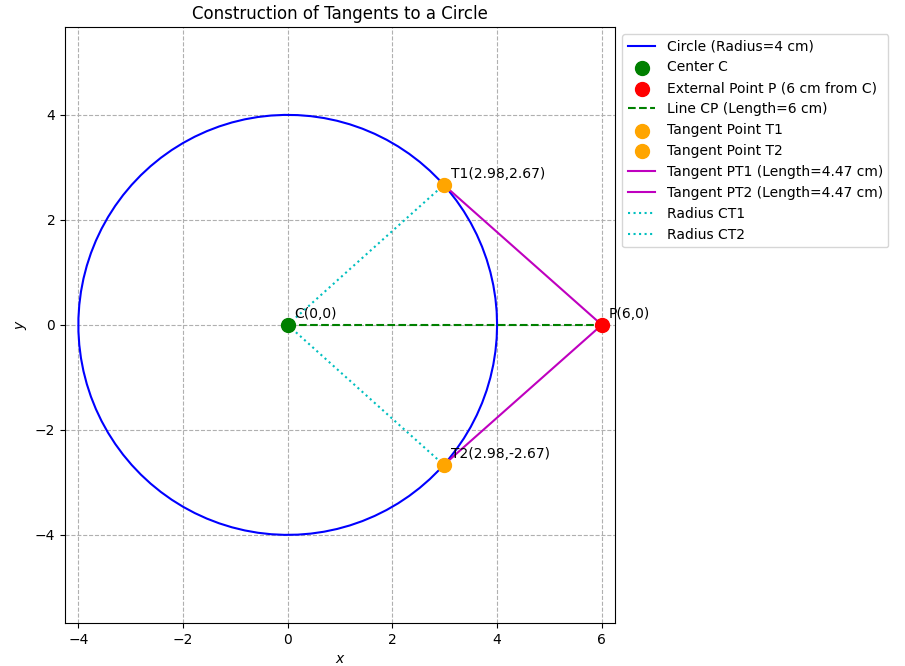
\includegraphics[width=0.8\columnwidth]{../figs/fig1.png}
\caption{}
\label{fig:1}
\end{figure}
\end{frame}

\begin{frame}{Plot by Python only}
\begin{figure}[H]
\centering
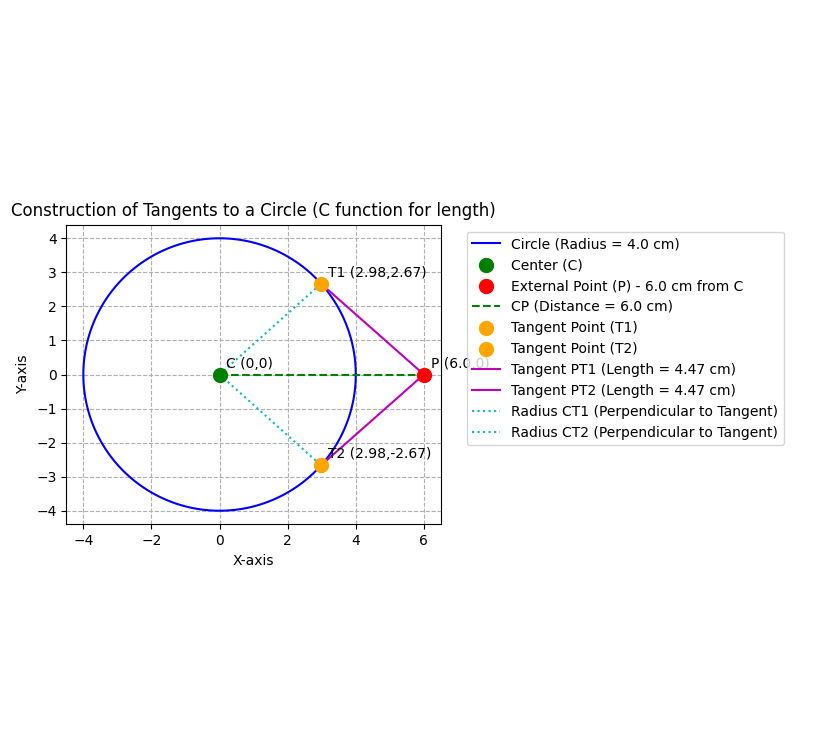
\includegraphics[width=0.7\columnwidth]{../figs/fig2.png}
\caption{}
\label{fig:2}
\end{figure}
\end{frame}

\end{document}
